\chapter{User Interface}
\label{chapter_ui}

This chapter, as apparent from its name, is considered as a reference for the MITHRA user interface.
%
The aim here is presenting the functions and variables which can be delivered to the MITHRA software and can be handled for a FEL simulation problem.
%
In what follows in this chapter, the defined language of MITHRA for writing a compatible job file is introduced.
%
This chapter can also be considered as a reference for the current capabilities of MITHRA and with time will be updated with the further improvement of the software capabilities.
%
\begin{description}
\item[\textbf{Iron Rule:}] parameters that are used for the solution of a specific electromagnetic problem are delivered to the code at only one single location, \emph{the job file}. This is indeed the only thing that the solver takes as an input parameter.
\end{description}
%
It should be noted that all the parameters in job file are given in the laboratory frame.
%
The Lorentz boost into the bunch rest frame will be done by the software automatically.

To run a job file using MITHRA, the following command should be written in the linux command line:

\begin{itemize}
	\item  {\textbf{\texttt{\small mpirun -np}}} "number of distributed processors" "MITHRA object file name" "job file name"
\end{itemize}

The transferred job file to the solver contains five main sections, each one defining an essential part of the electromagnetic problem.
%
These sections include:
%
\begin{enumerate}
	%
	\item {\tt \em \small MESH:} The parameters of the FDTD solver like the computational domain, cell sizes and time steps are set in this section.
	%
	\item {\tt \em \small BUNCH:} The required data to initialize the electron bunch in the computational domain is set in this section. In addition, the desired type of recording the bunch evolution is entered in this section by the user.
	%
	\item {\tt \em \small FIELD:} This section fulfills the same task as the previous section for the electromagnetic fields. The field initialization in case of a seeded FEL and the desired output type for the field evolution is given in this section to the software.
	%
	\item {\tt \em \small UNDULATOR:} This section introduces the different parameters of the undulator.
	%
	\item {\tt \em \small EXTERNAL-FIELD:} This section introduces the fields of some external components to the FEL interaction. It is relatively rare to have external components superimposed on the undulator field. However, such a possibility enables studying novel and advanced FEL cases.
	%
	\item {\tt \em \small FEL-OUTPUT:} The desired data related to the FEL radiation and how to record this data is set in this section.
\end{enumerate}
%
In the next subsections, we explain each part and the supported parameters, respectively.
%
To write comments in your job file use the sign "\#" at the beginning of the comment and the text will be commented to the end of the line.

\section{\texttt{MESH}}

As mentioned above, this part is dedicated to the determination of the FDTD/PIC parameters.
%
In Fig\,\ref{RefcardFig1}, a typical computation domain assumed in MITHRA is depicted.
%
\begin{figure}
\centering
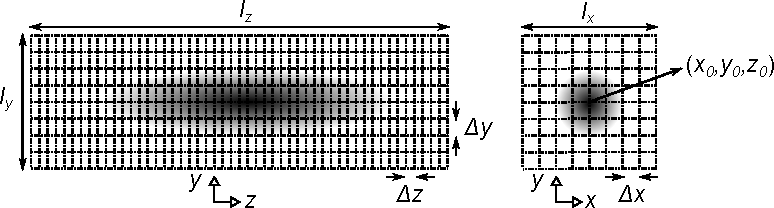
\includegraphics[width=5.0in]{./MITHRA_UI/Fig1.pdf}
\caption{The definition of the spatial mesh parameters in MITHRA}
\label{RefcardFig1}
\end{figure}
%
The mesh and update parameters of the solver are defined through the following ten parameters:
%
\begin{itemize}
	%
	\item {\tt \em \small length-scale} is the scaling of the length and all the spatial parameters in the job file. The capability to play with length scales is crucial to avoid working with very large or very small numbers.
	%
	\item {\tt \em \small time-scale} is the scaling of the time and all the temporal parameters in the job file. Similar to above, through this capability working with very large or very small numbers is avoided.
	%
	\item {\tt \em \small mesh-lengths} is a three dimensional vector equal to the lengths $(l_x,l_y,l_z)$ of the computational domain (\ref{RefcardFig1}) along the three Cartesian axes.
	%
	\item {\tt \em \small mesh-resolution} defines the length of one single grid cell or in other words the spatial discretization resolution of the FDTD mesh in the laboratory coordinate system $(\Delta x',\Delta y',\Delta z')$.
	%
	\item {\tt \em \small mesh-center} is the position of the central point of the computational rectangle, i.e. $(x_0',y_0',z_0')$ in Fig.\,\ref{RefcardFig1}.
	%
	\item {\tt \em \small total-time} is the total computation time in the scale given by the time scale. This is indeed the time it takes for the electron bunch to travel through the considered undulator length.
	%
	\item {\tt \em \small bunch-time-step} is the time step for updating the macro-particles' coordinates in the PIC solver.
	%
	\item {\tt \em \small mesh-truncation-order} is the truncation order of the absorbing boundary condition in the computational domain. This parameter can be either 1 or 2, representing the first order and second order absorbing boundary condition.
	%
	\item {\tt \em \small space-charge} is a boolean flag determining if the space-charge effect should be considered or not. If this flag is false, the scalar potential $\phi$ is zero throughout the calculation. Otherwise, the scalar potential is calculated using the corresponding Helmholtz equation.
	%
	\item {\tt \em \small solver} determines if the non-standard finite-difference (NSFD) algorithm should be used to remove the effects of numerical dispersion or the simulation should be done with a simple finite-difference (FD) algorithm. Default is the non-standard finite-difference.
\end{itemize}

The format of the {\tt \em \small MESH} group is:
%
\begin{Verbatim}[frame=single, fontsize=\small, tabsize=4, fontfamily=courier, fontseries=b, commandchars=\\\{\}, obeytabs]
MESH
\{
	length-scale				= < real | METER | DECIMETER | CENTIMETER | MILLIMETER | 
									MICROMETER | NANOMETER | ANGSTROM >
	time-scale					= < real | SECOND | MILLISECOND | MICROSECOND | NANOSECOND | 
									PICOSECOND | FEMTOSECOND |	ATTOSECOND >
	mesh-lengths				= < ( real, real, real ) >
	mesh-resolution		 		= < ( real, real, real ) >
	mesh-center				 	= < ( real, real, real ) >
	total-time					= < real >
	bunch-time-step		 		= < real >
	mesh-truncation-order 		= < 1 | 2 >
	space-charge  				= < true | false >
	solver						= < NSFD | FD >
\}
\end{Verbatim}
%%
An example of the computational mesh definition looks as the following:
%%
\begin{snugshade}
\begin{Verbatim}[fontsize=\small, tabsize=4, fontfamily=courier, fontseries=b, commandchars=\\\{\}, obeytabs]
MESH
\{
	length-scale 				 = MICROMETER
	time-scale					 = PICOSECOND
	mesh-lengths				 = ( 3200,  3200.0,    280.0)
	mesh-resolution				 = ( 50.0,    50.0,      0.1)
	mesh-center					 = ( 0.0,      0.0,      0.0)
	total-time 					 = 30000
	bunch-time-step				 = 1.6
	mesh-truncation-order		 = 2
	space-charge				 = false
	solver						 = NSFD
\}
\end{Verbatim}
\end{snugshade}
%
Note that there are some conditions, which should be fulfilled for the numerical integrator to obtain reliable dispersion-less results.
%
The software checks for these conditions before starting to solve the problem, if the conditions are violated the closest value to the given number meeting the violated conditions will be used.
%
Regarding the above parameters. the software checks for the stability condition $\sqrt{(\Delta z/\Delta x)^2+ (\Delta z/\Delta y)^2} < 1$, adapts the values of $\Delta x$ and $\Delta y$ accordingly, and finally sets the time step for field update equal to $\Delta z / c$.
%
In addition, the bunch update time step should be an integer fraction of the field time step to avoid redundant dispersion in the calculated values.
%
Therefore, the closest value to the given bunch time step, which satisfies the above criterion, will be chosen.

\section{\texttt{BUNCH}}

The section {\tt \small \em BUNCH} is the main part of the job file to establish the required data for the bunch input and output framework.
%
This section consists of four groups: (1) {\tt \em \small bunch-initialization}, (2) {\tt \em \small bunch-sampling}, (3) {\tt \em \small bunch-visualization}, and (4) {\tt \em \small bunch-profile}.
%
As apparent from the name the first group determines the set of parameters to initialize the bunch and the other three groups are dedicated to reporting the bunch evolution in different formats.
%
In what follows, the parameters in each group are introduced:

\begin{enumerate}
\item {\tt \small \em bunch-initialization:} This group mainly determines the parameters whose values are needed for initializing a bunch of electrons with different types. If several bunches are present in a simulation, this group should simply be repeated in the {\tt \small \em BUNCH} section. The set of values accepted in this group include:
%
\begin{itemize}
\item {\tt \small \em type} is the type of the bunch to be initialized in the computational domain. There are four bunch types supported by MITHRA:
\begin{enumerate}
	\item {\tt \small \em manual} initializes charges at the points specified by the position vector. At each appearance of this type of bunch only one single macro-particle will be initialized. Therefore, to have multiple manual initialization, the {\tt \small \em bunch-initialization} group should be repeated. Using the {\tt \small \em file} type is a better solution for high number of manual inputs. Alternatively, one can repeat the {\tt \small \em position} parameter to manually inject several particles.
	%
	\item {\tt \small \em ellipsoid} initializes charges with a given distribution over an ellipsoid defined by the {\tt \small \em sigma-position} parameter.
	%
	\item {\tt \small \em 3D-crystal} initializes multiple bunches on the points of a 3D crystal centered at the coordinate specified by the position vector and extends over the space by the number vector and the considered lattice constant. Each single bunch has a ellipsoid Gaussian property with the values read from the deviation parameters.
	%
	\item {\tt \small \em file} reads a list of 6D position and momentum coordinates from a file and initializes the macro-particles correspondingly in the solver. The format of the file that is read by MITHRA is a text ({\tt \small .txt}) file. In this file, each line presents the properties of one macro-particle that should be initialized in the code. In each line, six values corresponding to position of the macro-particle ($x, y, z$) and its normalized momentum ($\gamma\beta_x, \gamma\beta_y, \gamma\beta_z$) are written. This simple format is also the general format of all the bunch profiles produced by the MITHRA code.
\end{enumerate}
%
\item {\tt \small \em distribution} determines if the initialized particle distribution should have a uniform or Gaussian current profile. In MITHRA, the transverse distributions are always Gaussian, unless the bunch is given manually. This parameter merely affects the distribution along the traveling path, i.e. $z$.
%
\item {\tt \small \em number-of-particles} is the total number of particles (or macro-particles) considered in the bunch. The value should be a multiple of 4. Otherwise, the solver automatically changes the given value to the closest multiple of 4.
%
\item {\tt \small \em charge} is the total charge of the bunch in one electron charge unit. In other words, it stands for the total number of electrons in the bunch.
%
\item {\tt \small \em gamma} is the initial mean Lorentz factor of the bunch.
%
\item {\tt \small \em beta} is the initial mean normalized velocity of the particles, if it is not determined here the value will be calculated from the {\tt \small \em gamma} parameter, otherwise the same {\tt \small \em beta} will be used.
%
\item {\tt \small \em direction} is the average momentum direction of the bunch, i.e. $(\beta_x, \beta_y, \beta_z)/\beta$. In a typical FEL example, this parameter should be $(0, 0, 1)$.
%
\item {\tt \small \em position} is the central position of the bunch. This parameter can be repeated to initialize multiple bunches with similar profiles at different positions.
%
\item {\tt \small \em sigma-position} is the RMS deviation in position of the bunch, i.e. $(\sigma_x, \sigma_y, \sigma_z)$ for Gaussian distributions. $\sigma_z$ is half the bunch length for the uniform distribution.
%
\item {\tt \small \em sigma-momentum} is the RMS deviation in energy of the bunch, i.e. $(\sigma_{\gamma \beta_x}, \sigma_{\gamma \beta_y}, \sigma_{\gamma \beta_z})$.
%
\item {\tt \small \em numbers} is a parameter read only when the bunch type is a {\tt \small \em 3d-crystal} type. It is the number of bunch replication in the three directions.
%
\item {\tt \small \em lattice-constants} is a parameter read only when the bunch type is a {\tt \small \em 3d-crystal} type. It is the length of lattice constants of the crystal in the three directions.
%
\item {\tt \small \em transverse-truncation} determines a limit to transversely truncate the bunches. This factor brings the possibility to control particle initialization and prevents them from escaping out of the computational domain. The bunch initializer truncates the bunch at the given distance from the bunch center.
%
\item {\tt \small \em longitudinal-truncation} determines a limit to longitudinally truncate the bunches. This factor brings the possibility to control particle initialization and prevents them from escaping out of the computational domain. The bunch initializer truncates the bunch at the given distance from the bunch center.
%
\item {\tt \small \em bunching-factor} is a value larger than zero and less than one, which determines the bunching factor, i.e. $<e^{jk_uz}>$, of the initialized bunch.
%
\item {\tt \small \em bunching-factor-phase} is the initial phase of the bunching factor that is read in the parameter {\tt \small \em bunching-factor}.
%
\item {\tt \small \em shot-noise} is a boolean parameter that determines if the shot-noise should be introduced to the bunch initialization or not. To model, SASE FEL, this parameter should be set to {\tt \small \em true}.
%
\end{itemize}
%%
\item {\tt \small \em bunch-sampling:} This group defines the required parameters for saving the bunch properties with time. The bunch mean position, mean momentum, position spread, and momentum spread along the three Cartesian coordinates are saved respectively with time. There are different parameters required for this definition which include:
%
\begin{itemize}
	\item {\tt \small \em sample} is a boolean value determining if the bunch sampling should be activated.
	%
	\item {\tt \small \em base-name} is the file name (no suffix) with the required address of the file to save the output data.
	%
	\item {\tt \small \em directory} is the address where the above file should be saved. The file name with the address can also be given in the base-name section. The software eventually considers the combination of directory and base-name as the final complete file name.
	%
	\item {\tt \small \em rhythm} is a real value returning the rhythm of bunch sampling, i.e. the time interval between two consecutive sampling times.
\end{itemize}
%%
\item {\tt \small \em bunch-visualization:} This group defines the required parameters for visualizing the charge distribution in the whole computational domain. The output will be a set of {\tt \small \em .vtu} files at each time for each processor, which are connected with a set of {\tt \small \em .pvtu} files. They can be very nicely visualized using the open source ParaView package. There are different parameters required for this definition which include:
%
\begin{itemize}
	\item {\tt \small \em sample} is a boolean value determining if the charge visualization should be activated.
	%
	\item {\tt \small \em base-name} is the file name (no suffix) with the required address of the file to save the output data.
	%
	\item {\tt \small \em directory} is the address where the above file should be saved. The file name with the address can also be given in the base-name section. The software eventually considers the combination of directory and base-name as the final complete file name.
	%
	\item {\tt \small \em rhythm} is the rhythm of charge visualization, i.e. the time interval between two consecutive visualization times.
\end{itemize}
%
\item {\tt \small \em bunch-profile:} This group defines the required parameters for saving a histogram of the charges. It means that at a specific time instant the charge values, positions and momenta of all the particles (or macro-particles) will be written and saved in a file. The parameters entered by the user for saving the histogram include:
%
\begin{itemize}
	\item {\tt \small \em sample} is a boolean value determining if the writing of the histogram during the PIC simulations should be activated.
	%
	\item {\tt \small \em base-name} is the file name (no suffix) with the required address of the file to save the output data.
	%
	\item {\tt \small \em directory} is the address where the above file should be saved. The file name with the address can also be given in the base-name section. The software eventually considers the combination of directory and base-name as the final complete file name.
	%
	\item {\tt \small \em time} is the time instant for saving the histogram. If this needs to be done in several time instants, simply this line should be repeated with different time values.
	%
    \item {\tt \small \em rhythm} is the rhythm of writing the bunch profile, i.e. the time interval between two consecutive profiling times. If this value is nonzero, the sequence of times will be considered in addition to the specific time points given by the time variable.
\end{itemize}
\end{enumerate}

The format of the {\tt \small \em BUNCH} group is (The repeatable variables are shown in red):
%
\begin{Verbatim}[frame=single, fontsize=\small, tabsize=4, fontfamily=courier, fontseries=b, commandchars=\\\{\}, obeytabs]
BUNCH
\{
	\textcolor{red}{bunch-initialization}
	\textcolor{red}{\{}
		type  					 = < manual | ellipsoid | 3D-crystal | file >
		distribution  			 = < uniform | gaussian >
		charge  				 = < real >
		number-of-particles		 = < int >
		gamma  					 = < real >
		beta  					 = < real >
		direction  				 = < ( real, real, real ) >
		\textcolor{red}{position}				 \textcolor{red}{= < ( real, real, real ) >}
		sigma-position  		 = < ( real, real, real ) >
		sigma-momentum  		 = < ( real, real, real ) >
		numbers					 = < ( int, int, int ) >
		lattice-constants		 = < ( real, real, real ) >
		transverse-truncation	 = < real >
		longitudinal-truncation  = < real >
		bunching-factor			 = < real between 0 and 1 >
		bunching-factor-phase	 = < real >
		shot-noise  			 = < true | false >
	\textcolor{red}{\}}

	bunch-sampling
	\{
		sample  				 = < true | false >
		directory  				 = < /path/to/location >
		base-name  				 = < string >
		rhythm  				 = < real >
	\}

	bunch-visualization
	\{
		sample  				 = < true | false >
		directory  				 = < /path/to/location >
		base-name  				 = < string >
		rhythm  				 = < real >
	\}

	bunch-profile
	\{
		sample  				 = < true | false >
		directory  				 = < /path/to/location >
		base-name  				 = < string >
		\textcolor{red}{time}					\textcolor{red}{ = < real >}
		rhythm  				 = < real >
	\}
\}
\end{Verbatim}
%
An example of the bunch category definition looks as the following:
%
\begin{snugshade}
\begin{Verbatim}[fontsize=\small, tabsize=4, fontfamily=courier, fontseries=b, commandchars=\\\{\}, obeytabs]
BUNCH
\{
	bunch-initialization
	\{
		type					  = ellipsoid
		distribution			  = uniform
		charge					  = 1.846e8
		number-of-particles 	  = 131072
		gamma					  = 100.41
		direction				  = ( 0.0, 0.0, 1.0)
		position				  = ( 0.0, 0.0, 0.0)
		sigma-position			  = ( 260.0, 260.0, 50.25)
		sigma-momentum			  = ( 1.0e-8, 1.0e-8, 100.41e-4)
		transverse-truncation	  = 1040.0
		longitudinal-truncation	  = 90.0
		bunching-factor			  = 0.01
		bunching-factor-phase	  = 0.0
		shot-noise				  = false
  	\}

	bunch-sampling
	\{
		sample					  = false
		directory				  = ./
		base-name				  = bunch-sampling/bunch
		rhythm					  = 3.2
	\}
	
	bunch-visualization
	\{
		 sample					  = true
		 directory				  = ./
		 base-name				  = bunch-visualization/bunch
		 rhythm					  = 32
	\}
	
	bunch-profile
	\{
		 sample					  = false
		 directory				  = ./
		 base-name				  = bunch-profile/bunch
		 time					  = 5000
		 time					  = 10000
		 time					  = 15000
		 time					  = 20000
		 time					  = 25000
		 time					  = 30000
	\}
\}
\end{Verbatim}
\end{snugshade}

\section{\texttt{FIELD}}

In section {\tt \small \em FIELD}, the required data for the input and output framework of the field in the FDTD algorithm is produced.
%
This section consists of four groups: (1) {\tt \small \em field-initialization}, (2) {\tt \small \em field-sampling}, (3) {\tt \small \em field-visualization}, and (4) {\tt \small \em field-profile}.
%
As apparent from the name, the first group determines the set of parameters to initialize the field and the other three groups are dedicated to reporting the field propagation in different formats.
%
In what follows, the parameters in each group are introduced:

\begin{enumerate}
\item {\tt \small \em field-initialization:} This group mainly determines the parameters whose values are needed for initializing a field excitation entering the computational domain. The excitation may have different types. This group is where a seed can be added to the simulations to simulate a seeded-FEL problem. The set of values accepted in this group include:
%
\begin{itemize}
	\item {\tt \small \em type} is the type of the excitation. The accepted excitation types in MITHRA include plane wave, confined plane-wave, and Gaussian beam. A confined plane-wave is a plane-wave that introduces fields to the particle only over an ellipse determined by beam radii.
	%
	\item {\tt \small \em position} is the reference position of the excitation. It is the reference position of the plane wave propagation in the plane-wave excitation and the focusing point in the Gaussian beam excitation. The coordinate system for this position vector is the same as for bunch position vector. Typically, the focal point or the reference position of the seed is given with respect to the undulator begin. Therefore, special care should be exercised with this position vector;
	If the reference position with respect to undulator begin is $z_0$, then the value for seed reference position should be given as $z_0 + l_z + 10\lambda_X$, where $l_z$ is the {\tt \small \em longitudinal truncation} value and $\lambda_X$ is the radiation wavelength.
	%
	\item {\tt \small \em direction} is the propagation direction of the excitation in the plane-wave and Gaussian beam types.
	%
	\item {\tt \small \em polarization} is the polarization of the incoming excitation and is used by both plane-wave and Gaussian-beam types.
	%
	\item {\tt \small \em radius-parallel} is the Rayleigh radius (beam waist) of the Gaussian beam in the direction parallel to the polarization. For the confined plane-wave it is the radius of the ellipse along the polarization direction confining the plane wave.
	%
	\item {\tt \small \em radius-perpendicular} is the Rayleigh radius (beam waist) of the Gaussian beam in the direction perpendicular to the polarization. For the confined plane-wave it is the radius of the ellipse perpendicular to the polarization direction confining the plane-wave.
	%
	\item {\tt \small \em signal-type} determines the time signature of the signal exciting the fields according to the particular type. The accepted signal types in MITHRA include modulated Neumann, modulated Gaussian, modulated secant hyperbolic and the sinusoidal pulse. The equation representing the time domain variation of each pulse is as follows:
	%
	\begin{equation}
	\label{signalTypes}
	\renewcommand{\arraystretch}{1.5}
	\begin{array}{lrcl}
	\mbox{modulated Neumann:}  \qquad & f(t,t_0,\phi_\mathrm{CEP}) & = & \displaystyle - A_0 4 \ln 2 \: \cos( 2 \pi f (t - t_0) + \phi_\mathrm{CEP} ) \frac{t - t_0}{\tau^2} e^{-2 \ln 2 \: (t - t_0)^2/\tau^2 } \\
	\mbox{modulated Gaussian:} \qquad & f(t,t_0,\phi_\mathrm{CEP}) & = & \displaystyle A_0 \cos( 2 \pi f (t - t_0) + \phi_\mathrm{CEP} ) e^{-2 \ln 2 \: (t - t_0)^2/\tau^2 } \\
	\mbox{modulated hyperbolic secant:} \qquad & f(t,t_0,\phi_\mathrm{CEP}) & = & \displaystyle A_0 \cos( 2 \pi f (t - t_0) + \phi_\mathrm{CEP} ) \frac{1}{\cosh ( (t - t_0)/\tau ) } \\
	\mbox{sinusoidal pulse:}   \qquad & f(t,t_0,\phi_\mathrm{CEP}) & = & \displaystyle \left\{ \begin{array}{ll} A_0 \cos( 2 \pi f (t - t_0) + \phi_\mathrm{CEP} ) e^{-2 \ln 2 \: (t - t_0)^2/\tau^2 } & t \leq t_0 \\ A_0 \cos( 2 \pi f (t - t_0) + \phi_\mathrm{CEP} ) & t > t_0 \end{array} \right.
	\end{array}
	\end{equation}
	%
	\item {\tt \small \em strength-parameter} is the normalized amplitude $a_0 = e A_0 / m_ec $ of the beam.
	%
	\item {\tt \small \em offset} is the distance offset of the signal $ct_0$ with respect to the reference position.
	%
	\item {\tt \small \em pulse-length} is the pulse duration of the signal in length units $c\tau$. The pulse duration is defined as the interval in which the pulse intensity is larger than half the maximum intensity of the pulse, i.e. FWHM of the intensity.
	%
	\item {\tt \small \em wavelength} is the modulation wavelength $\lambda_0$ of the modulated signal.
	%
	\item {\tt \small \em CEP} is the carrier envelope phase $\phi_{\mathrm{CEP}}$ of the modulated signal in degrees.
\end{itemize}
%
\item {\tt \small \em field-sampling:} This group defines the required parameters for saving the field value at specific points with time. There are different parameters required for this definition which include:
%
\begin{itemize}
	\item {\tt \small \em sample} is a boolean value determining if the field sampling should be activated.
	%
	\item {\tt \small \em type} determines if the field should be sampled at the given points ({\tt \small \em at-point}) or the field should be sampled at the points over a line ({\tt \small \em over-line}).
	%
	\item {\tt \small \em field} determines which electromagnetic field is to be sampled. The available options are the electric field, magnetic field, magnetic vector potential, scalar electric potential, charge and current. This item can be repeated to assign several fields for the sampling. In the text file, the fields appear in columns with the same order as given in this group.
	%
	\item {\tt \small \em base-name} is the file name (no suffix) with the required address of the file to save the output data.
	%
	\item {\tt \small \em directory} is the address where the above file should be saved. The file name with the address can also be given in the base-name section. The software eventually considers the combination of directory and base-name as the final complete file name.
	%
	\item {\tt \small \em rhythm} is a real value determining the rhythm of field sampling, i.e. the time interval between two consecutive sampling times.
	%
	\item {\tt \small \em position} is the coordinate of the points where the fields should be sampled. By repeating this line any number of points can be added to the set of sampling locations. This option is merely used when the sampling type is set to {\tt \small \em at-point}.
	%
	\item {\tt \small \em line-begin} defines the position of the line begin over which the fields should be sampled and is used when the sampling type is set to {\tt \small \em over-line}.
	%
	\item {\tt \small \em line-end} defines the position of the line end over which the fields should be sampled and is used when the sampling type is set to {\tt \small \em over-line}.
	%
	\item {\tt \small \em number-of-points} is the number of points between line-begin and line-end for field-sampling. This value is used when the sampling type is set to {\tt \small \em over-line}.
\end{itemize}
%%
\item {\tt \small \em field-visualization:} This group defines the required parameters for visualizing the fields in the whole computational domain. The output will be a set of \texttt{.vtu} files at each time for each processor which are connected with a set of \texttt{.pvtu} files. They can be very nicely visualized using the open source ParaView package. To enable various visualizations, this group can be repeated in the job file. There are different parameters required for this definition which include:
%
\begin{itemize}
	\item {\tt \small \em sample} is a boolean value determining if the field visualization should be activated.
	%
	\item {\tt \small \em base-name} is the file name (no suffix) with the required address of the file to save the output data.
	%
	\item {\tt \small \em directory} is the address where the above file should be saved. The file name with the address can also be given in the base-name section. The software eventually considers the combination of directory and base-name as the final complete file name.
	%
	\item {\tt \small \em type} is the type of visualization and mainly decides if the visualization is 2D ({\tt \small \em in-plane}) or 3D ({\tt \small \em all-domain}).
	%
	\item {\tt \small \em plane} is the plane of field-visualization if the visualization is to be done over a 2D plane. This parameter is read only if {\tt \small \em type} is set to {\tt \small \em in-plane}.
	%
	\item {\tt \small \em rhythm} is the rhythm of field visualization, i.e. the time interval between two consecutive visualization instants.
	%
	\item {\tt \small \em field} determines which electromagnetic field is to be visualized. The available options are the electric field, magnetic field, magnetic vector potential, scalar electric potential, charge and current. This item can be repeated to assign several fields for the sampling. In the vtk file, the fields appear with the same order. To make the output compatible with the visualizer ParaView, it is most suitable if three consistent parameters are given here.
\end{itemize}
%%
\item {\tt \small \em field-profile:} This group defines the required parameters for saving a histogram of the field over the whole computational domain. It means that at a specific time instant the field values and the corresponding positions at all the grid points will be written and saved in a text file. The parameters entered by the user for saving the histogram include:
%
\begin{itemize}
	\item {\tt \small \em sample} is a boolean value determining if the writing of the histogram during the FDTD simulations should be activated.
	%
	\item {\tt \small \em base-name} is the file name (no suffix) with the required address of the file to save the output data.
	%
	\item {\tt \small \em directory} is the address where the above file should be saved. The file name with the address can also be given in the base-name section. The software eventually considers the combination of directory and base-name as the final complete file name.
	%
	\item {\tt \small \em time} is the time instant for saving the histogram. If this needs to be done in several time instants, simply this line should be repeated with different time values.
	%
	\item {\tt \small \em rhythm} is the rhythm of field profiling, i.e. the time interval between two consecutive profiling times. Both rhythmic profiling and saving the fields at specific times can be given to the software.
	%
	\item {\tt \small \em field} determines which electromagnetic field is to be profiled. The available options are the electric field, magnetic field, magnetic vector potential, scalar electric potential, charge and current. This item can be repeated to assign several fields for the sampling. In the text file, the fields appear with the same order.
\end{itemize}
\end{enumerate}

The format of the {\tt \small \em FIELD} group is (The repeatable variables are shown in red):
%
\begin{Verbatim}[frame=single, fontsize=\small, tabsize=4, fontfamily=courier, fontseries=b, commandchars=\\\{\}, obeytabs]
FIELD
\{
	field-initialization
	\{
		type  					 = < plane-wave | confined-plane-wave | gaussian-beam >
		position  				 = < ( real, real, real ) >
		direction  				 = < ( real, real, real ) >
		polarization  			 = < ( real, real, real ) >
		radius-parallel  		 = < real >
		radius-perpendicular  	 = < real >
		signal-type  			 = < neumann | gaussian | secant-hyperbolic | flat-top >
		strength-parameter  	 = < real >
		offset  				 = < real >
		pulse-length  			 = < real >
		wavelength  			 = < real >
		CEP  					 = < real >
	\}

	field-sampling
	\{
		sample  				 = < true | false >
		type  					 = < over-line | at-point >
		\textcolor{red}{field} 					\textcolor{red}{ = < Ex | Ey | Ez | Bx | By | Bz | Ax | Ay | Az | Jx | Jy | Jz | }
									 \textcolor{red}{F  | Q >}
		directory  				 = < /path/to/location >
		base-name  				 = < string >
		rhythm  				 = < real >
		\textcolor{red}{position}  				 \textcolor{red}{= < ( real, real, real ) >}
		line-begin  			 = < ( real, real, real ) >
		line-end  				 = < ( real, real, real ) >
		number-of-points  		 = < int >
	\}

	\textcolor{red}{field-visualization}
	\textcolor{red}{\{}
		sample  				 = < true | false >
		type					 = < in-plane | all-domain >
		plane					 = < xy | yz | xz >
		position  				 = < ( real, real, real ) >
		\textcolor{red}{field} 					\textcolor{red}{ = < Ex | Ey | Ez | Bx | By | Bz | Ax | Ay | Az | Jx | Jy | Jz | }
									 \textcolor{red}{F  | Q >}
		directory  				 = < /path/to/location >
		base-name  				 = < string >
		rhythm  				 = < real >
	\textcolor{red}{\}}

	field-profile
	\{
		sample  				 = < true | false >
		\textcolor{red}{field} 					\textcolor{red}{ = < Ex | Ey | Ez | Bx | By | Bz | Ax | Ay | Az | Jx | Jy | Jz | }
									 \textcolor{red}{F  | Q >}
		directory  				 = < /path/to/location >
		base-name  				 = < string >
		rhythm  				 = < real >
		\textcolor{red}{time}  					 \textcolor{red}{= < real >}
	\}
\}
\end{Verbatim}
%
An example of the field category definition looks as the following:
%
\begin{snugshade}
\begin{Verbatim}[fontsize=\small, tabsize=4, fontfamily=courier, fontseries=b, commandchars=\\\{\}, obeytabs]
FIELD
\{
	field-initialization
	\{
		type					  = gaussian-beam
		position				  = ( 0.0, 0.0, -2500.0)
		direction				  = ( 0.0, 0.0, 1.0)
		polarization			  = ( 0.0, 1.0, 0.0)
		radius-parallel			  = 0.5
		radius-perpendicular	  = 0.5
		strength-parameter		  = 0.0
		signal-type				  = gaussian
		offset					  = 0.00
		pulse-length			  = 1.00
		wavelength				  = 0.0
		CEP						  = 0.0
	\}
	
	field-sampling
	\{
		sample					  = true
		type					  = at-point
		field					  = Ex
		field					  = Ey
		field					  = Ez
		directory				  = ./
		base-name				  = field-sampling/field
		rhythm					  = 3.2
		position				  = (0.0, 0.0, 110.0)
	\}
	
	field-visualization
	\{
		sample					  = true
		field					  = Ex
		field					  = Ey
		field					  = Ez
		field					  = Q
		directory				  = ./
		base-name				  = field-visualization/field
		rhythm					  = 32
	\}
	
	field-profile
	\{
		sample					  = false
		field					  = Ex
		field					  = Ey
		field					  = Ez
		directory				  = ./
		base-name				  = field-profile/field
		rhythm					  = 80
	\}
\}
\end{Verbatim}
\end{snugshade}

\section{\texttt{UNDULATOR}}

In section \texttt{UNDULATOR}, the properties of the undulator considered in the FEL problem are introduced.
%
The parameters for establishing undulator fields are obtained in various groups.
%
These groups contain the already implemented undulator types and get updated with time.
%
By adding additional groups, the fileds of these undulators are superposed.
%
Note that the reference undulator for initializing bunches or setting the electron rest frame is the first undulator given in the list.

\begin{enumerate}
%
\item {\tt \small \em static-undulator:} This group mainly determines the parameters for defining a static undulator. The set of values accepted in this group include:
%
\begin{itemize}
	\item {\tt \small \em undulator-parameter} is the undulator parameter of the undulator, i.e. the so-called K parameter.
	%
	\item {\tt \small \em period} is the period of the undulator in the given length-scale determined in the mesh class.
	%
	\item {\tt \small \em length} is an integer returning the total length of the undulator in one period scale. In other words, it determines the number of undulator periods in the module.
	%
    \item {\tt \small \em polarization-angle} is the angle between the magnetic field polarization and the $x$-axis in degrees.
    %
    \item {\tt \small \em offset} determines the point where the beginning of undulator resides. For the first undulator, it is automatically set to zero.
    %
    \item {\tt \small \em distance-to-bunch-head} determines the distance between the undulator entrance and the bunch head at the initialization time. This distance is needed to avoid particles experiencing a sudden change in the undulator field. The value of this parameter is by default two undulator periods.
    %
\end{itemize}
%
\item {\tt \small \em static-undulator-array:} This group determines the required parameters for defining an array of static undulators. The set of values accepted in this group include:
%
\begin{itemize}
	\item {\tt \small \em undulator-parameter} is the undulator parameter of the undulators, i.e. the so-called K parameter. For a non-zero tapering parameter, this value corresponds to the K-parameter of the first undulator.
	%
	\item {\tt \small \em period} is the period of the undulators in the given length-scale determined in the mesh class.
	%
	\item {\tt \small \em length} is an integer returning the total length of the undulator in one period scale. In other words, it determines the number of undulator periods in the module.
	%
	\item {\tt \small \em polarization-angle} is the angle between the magnetic field polarization and the $x$-axis in degrees.
	%
	\item {\tt \small \em distance-to-bunch-head} is the initial distance between the head of the bunch and the beginning of the undulator. By default, a distance of two undulator periods is considered in MITHRA.
	%
	\item {\tt \small \em gap} determines the gap between the adjacent undulators.
	%
    \item {\tt \small \em number} is the total number of undulator modules in the array.
    %
    \item {\tt \small \em tapering-parameter} is the tapering parameter of the undulator array, i.e. $\delta K$ in $K_i=K_0+i \delta K$ giving the K parameters of the $i$'th undulator module.
    %
    \item {\tt \small \em distance-to-bunch-head} determines the distance between the {\em first} undulator entrance and the bunch head at the initialization time. This distance is needed to avoid particles experiencing a sudden change in the undulator field. The value of this parameter is by default two undulator periods.
    %
\end{itemize}
%
\item {\tt \small \em optical-undulator:} This group mainly determines the parameters for defining an optical undulator. The set of values accepted in this group include:
%
\begin{itemize}
	\item {\tt \small \em beam-type} is the type of the pulse for an optical undulator. The accepted undulator beam types in MITHRA include plane wave, confined plane-wave, and Gaussian beam. A confined plane-wave is a plane-wave that introduces fields to the particle only over an ellipse determined by beam waist.
	%
	\item {\tt \small \em position} is the reference position of the undulator. It is the reference position of the plane-wave propagation in the plane-wave undulator and the focusing point in the Gaussian beam undulator.
	%
	\item {\tt \small \em direction} is the propagation direction of the optical undulator in the plane-wave and Gaussian beam types.
	%
	\item {\tt \small \em polarization} is the polarization of the undulator and is used by both plane-wave and Gaussian beam types.
	%
	\item {\tt \small \em radius-parallel} is the Rayleigh radius (beam waist) of the Gaussian beam in the direction parallel to the polarization. For the confined plane-wave it is the radius of the ellipse along the polarization direction confining the plane-wave.
	%
	\item {\tt \small \em radius-perpendicular} is the Rayleigh radius (beam waist) of the Gaussian beam in the direction perpendicular to the polarization. For the confined plane-wave it is the radius of the ellipse perpendicular to the polarization direction confining the plane-wave.
	%
	\item {\tt \small \em signal-type} determines the time signature of the undulator. The accepted signal types in MITHRA are listed in the field section. Here, the same set of signal can be given as an undulator envelope.
	%
	\item {\tt \small \em strength-parameter} is the normalized amplitude $a_0 = e A_0 / m_ec $ of the undulator, which is equivalent to the undulator-parameter in the static case.
	%
	\item {\tt \small \em offset} is the distance offset of the signal $ct_0$. The user can play with this parameter and also the reference position to control the arrival time of the pulse on the bunch. By default, MITHRA considers a distance equal to 10 undulator period between the pulse begin and the head of the bunch.
	%
	\item {\tt \small \em pulse-length} is the pulse duration of the signal in length units $c\tau$. The pulse duration is defined as the interval in which the pulse intensity is larger than half the maximum intensity of the pulse, i.e. FWHM of the intensity.
	%
	\item {\tt \small \em wavelength} is the modulation wavelength $\lambda_0$ of the modulated signal.
	%
	\item {\tt \small \em CEP} is the carrier envelope phase $\phi_{\mathrm{CEP}}$ of the modulated signal.
\end{itemize}
%
\end{enumerate}

The format of the \texttt{UNDULATOR} group is (the read groups are repeatable groups):
%
\begin{Verbatim}[frame=single, fontsize=\small, tabsize=4, fontfamily=courier, fontseries=b, commandchars=\\\{\}, obeytabs]
UNDULATOR
\{
	\textcolor{red}{static-undulator}
	\textcolor{red}{\{}
		undulator-parameter		  = < real >
		period					  = < real >
		length					  = < int >
		polarization-angle		  = < real >
		offset					  = < real >
		distance-to-bunch-head 	  = < real >
	\textcolor{red}{\}}

	\textcolor{red}{static-undulator-array}
	\textcolor{red}{\{}
		undulator-parameter		  = < real >
		period					  = < real >
		length					  = < int >
		polarization-angle		  = < real >
		gap						  = < real >
		number					  = < int >
		tapering-parameter		  = < real >
		distance-to-bunch-head    = < real >
	\textcolor{red}{\}}

	\textcolor{red}{optical-undulator}
	\textcolor{red}{\{}
		beam-type				  = < plane-wave | confined-plane-wave | gaussian-beam >
		position				  = < ( real, real, real ) >
		direction				  = < ( real, real, real ) >
		polarization			  = < ( real, real, real ) >
		radius-parallel			  = < real >
		radius-perpendicular	  = < real >
		signal-type				  = < neumann | gaussian | secant-hyperbolic | flat-top >
		strength-parameter		  = < real >
		offset					  = < real >
		pulse-length			  = < real >
		wavelength				  = < real >
		CEP						  = < real >
	\textcolor{red}{\}}
\}
\end{Verbatim}
%
As explained before, MITHRA always initializes the bunch outside the undulator.
%
It may be already noticed that there exists no option to determine the beginning of the first static undulator with respect to the bunch, because MITHRA ignores this parameter for the first undulator.
%
This value is automatically set by the solver, to avoid particle initialization inside the undulator.
%
For the optical undulator type, the user should control this effect through the parameter offset.
%
An example of the undulator category definition looks as the following:
%
\begin{snugshade}
\begin{Verbatim}[fontsize=\small, tabsize=4, fontfamily=courier, fontseries=b, commandchars=\\\{\}, obeytabs]
UNDULATOR
\{
	static-undulator
	\{
		undulator-parameter		  = 1.417
    	period					  = 3.0e4
    	length					  = 300
    	polarization-angle		  = 0.0
    	offset					  = 0.0
    \}
\}
\end{Verbatim}
\end{snugshade}
%
An instance of optical undulator definition reads as follows:
%
\begin{snugshade}
\begin{Verbatim}[fontsize=\small, tabsize=4, fontfamily=courier, fontseries=b, commandchars=\\\{\}, obeytabs]
UNDULATOR
\{
	optical-undulator
	\{
		beam-type				  = plane-wave
		position				  = ( 0.0, 0.0, 0.0 )
		direction				  = ( 0.0, 0.0,-1.0 )
		polarization			  = ( 0.0, 1.0, 0.0 )
		strength-parameter		  = 0.5
		signal-type				  = flat-top
		wavelength				  = 1.0e3
		pulse-length			  = 1200.0e3
		offset					  = 600118.0
		CEP						  = 0.0
  \}
\}
\end{Verbatim}
\end{snugshade}

\section{\texttt{EXTERNAL-FIELD}}

The parameters for defining fields of additional components during the wiggling process are given to the solver in this section.
%
This part of the solver will be updated depending on the projects where MITHRA is used for modelling the interaction.
%
Put differently, the components used in the project over the undulator section in each project will be implemented in this section.
%
The current version of MITHRA accepts the following set of external fields:

\begin{enumerate}
%
\item {\tt \small \em electromagnetic-wave:} This group mainly determines the parameters for superposing the field of an electromagnetic beam over the undulator section. This external field in principle fulfills the same thing as a general seed in the FEL interaction. However, if the seed is defined as an external plane-wave, the output radiation does not include the field of seeded beam. In other words, it starts from a zero initial radiation. This group can be repeated to superpose a number of plane waves over each other during the interaction. The set of values accepted in this group include:
%
\begin{itemize}
	%
    \item {\tt \small \em beam-type} is the type of the beam. The accepted excitation types in MITHRA include plane-wave, confined plane-wave and Gaussian beam. A confined plane-wave is a plane-wave that introduces fields to the particle only over an ellipse determined by beam radii.
    %
    \item {\tt \small \em position} is the reference position of the excitation. It is the reference position of the plane-wave propagation in the plane-wave excitation and the focusing point in the Gaussian beam excitation.
    %
	\item {\tt \small \em direction} is the propagation direction of the excitation in the plane-wave and Gaussian beam types.
	%
	\item {\tt \small \em polarization} is the polarization of the incoming excitation and is used by both plane-wave and Gaussian beam types.
	%
	\item {\tt \small \em radius-parallel} is the Rayleigh radius (beam waist) of the Gaussian beam in the direction parallel to the polarization. For the confined plane-wave, it is the radius of the ellipse along the polarization direction confining the plane-wave.
	%
	\item {\tt \small \em radius-perpendicular} is the Rayleigh radius (beam waist) of the Gaussian beam in the direction perpendicular to the polarization. For the confined plane-wave, it is the radius of the ellipse perpendicular to the polarization direction confining the plane-wave.
	%
	\item {\tt \small \em signal-type} determines the time signature of the signal exciting the fields according to the particular type. The accepted signal types in MITHRA include modulated Neumann, modulated Gaussian, modulated secant-hyperbolic and the sinusoidal pulse. The equation representing the time domain variation of each pulse is as follows:
	%
	\begin{equation}
	\renewcommand{\arraystretch}{1.5}
	\begin{array}{lrcl}
	\mbox{modulated Neumann:}  \qquad & f(t) & = & \displaystyle - A_0 4 \ln 2 \: \cos( 2 \pi f (t - t_0) + \phi_\mathrm{CEP} ) \frac{t - t_0}{\tau^2} e^{-2 \ln 2 \: (t - t_0)^2/\tau^2 } \\
	\mbox{modulated Gaussian:} \qquad & f(t) & = & \displaystyle A_0 \cos( 2 \pi f (t - t_0) + \phi_\mathrm{CEP} ) e^{-2 \ln 2 \: (t - t_0)^2/\tau^2 } \\
	\mbox{modulated hyperbolic secant:} \qquad & f(t) & = & \displaystyle A_0 \cos( 2 \pi f (t - t_0) + \phi_\mathrm{CEP} ) \frac{1}{\cosh ( (t - t_0)/\tau ) } \\
	\mbox{sinusoidal pulse:}   \qquad & f(t) & = & \displaystyle \left\{ \begin{array}{ll} A_0 \cos( 2 \pi f (t - t_0) + \phi_\mathrm{CEP} ) e^{-2 \ln 2 \: (t - t_0)^2/\tau^2 } & t \leq t_0 \\ A_0 \cos( 2 \pi f (t - t_0) + \phi_\mathrm{CEP} ) & t > t_0 \end{array} \right.
	\end{array}
	\end{equation}
	\item {\tt \small \em strength-parameter} is the normalized amplitude $a_0 = e A_0 / m_ec $ of the beam.
	%
	\item {\tt \small \em offset} is the distance offset of the signal $ct_0$.
	%
	\item {\tt \small \em pulse-length} is the pulse duration of the signal in length units $c\tau$. The pulse duration is defined as the interval in which the pulse intensity is larger than half the maximum intensity of the pulse, i.e. FWHM of the intensity.
	%
	\item {\tt \small \em wavelength} is the modulation wavelength $\lambda_0$ of the modulated signal.
	%
	\item {\tt \small \em CEP} is the carrier envelope phase $\phi_{\mathrm{CEP}}$ of the modulated signal.
	%
\end{itemize}
\end{enumerate}

The format of the \texttt{FIELD} group is:
%%
\begin{Verbatim}[frame=single, fontsize=\small, tabsize=4, fontfamily=courier, fontseries=b, commandchars=\\\{\}, obeytabs]
EXTERNAL-FIELD
\{
	\textcolor{red}{electromagnetic-wave}
	\textcolor{red}{\{}
		beam-type				  = < plane-wave | confined-plane-wave | gaussian-beam >
		position				  = < ( real, real, real ) >
		direction				  = < ( real, real, real ) >
		polarization			  = < ( real, real, real ) >
		radius-parallel			  = < real >
		radius-perpendicular	  = < real >
		signal-type				  = < neumann | gaussian | secant-hyperbolic | flat-top >
		strength-parameter		  = < real >
		offset					  = < real >
		pulse-length			  = < real >
		wavelength				  = < real >
		CEP						  = < real >
	\textcolor{red}{\}}
\}
\end{Verbatim}

An example of the external field definition looks as the following:
%
\begin{snugshade}
\begin{Verbatim}[fontsize=\small, tabsize=4, fontfamily=courier, fontseries=b, commandchars=\\\{\}, obeytabs]
EXTERNAL-FIELD
\{
	electromagnetic-wave
	\{
		beam-type				  = plane-wave
		position				  = ( 0.0, 0.0, 0.0)
    	direction				  = ( 0.0, 1.0, 0.0)
    	polarization			  = ( 0.0, 0.0, 1.0)
    	strength-parameter		  = 1.0
    	signal-type				  = flat-top
    	offset					  = 0.00
    	pulse-length			  = 1.00
    	wavelength				  = 0.0
    	CEP						  = 0.0
	\}
	
	electromagnetic-wave
	\{
		beam-type				  = plane-wave
		position				  = ( 0.0, 0.0, 0.0)
		direction				  = ( 0.0,-1.0, 0.0)
		polarization			  = ( 0.0, 0.0, 1.0)
		strength-parameter		  = 1.0
		signal-type				  = flat-top
		offset					  = 0.00
		pulse-length			  = 1.00
		wavelength				  = 0.0
		CEP						  = 0.0
	\}
\}
\end{Verbatim}
\end{snugshade}
%

\section{\texttt{FEL-OUTPUT}}

The typical parameters for a free electron laser instrument are calculated from the radiated fields using the parameter definitions at this section.
%
Currently, there are three groups implemented in MITHRA, for computation of radiated power, visualization of this power on a detector in front of the bunch, and visualization of the bunch profile in the lab frame by recording the particles that are intercepted by screens placed along the z-axis.
%
In what follows, the parameters in each group are introduced:

\begin{enumerate}
%
\item {\tt \small \em radiation-power:} This group mainly determines the parameters whose values are needed for calculating the radiation power from the field distribution. The output is a .txt file with the first column the time point and the second column the radiated power at the given point. For multiple points the column is repeated. If multiple frequencies are given, there will be several rows with similar time value listing the radiated power with different wavelengths. This group can be repeated to obtain various files for different output definitions. 
%
The set of values accepted in this group include:
%
\begin{itemize}
	\item {\tt \small \em sample} is a boolean parameter which activates the computation of the total radiated power at each instant.
	%
	\item {\tt \small \em base-name} is the file name (no suffix) with the required address of the file to save the output data.
	%
	\item {\tt \small \em directory} is the address where the above file should be saved. The file name with the address can also be given in the base-name section. The software eventually considers the combination of directory and base-name as the final complete file name.
	%
	\item {\tt \small \em type} determines if the radiated power should be sampled at given distances from the bunch ({\tt \small \em at-point}) or should be sampled at the points over a line ({\tt \small \em over-line}).
	%
	\item {\tt \small \em plane-position} gives the total distance from the bunch where a sampling plate to capture the whole radiated power will be placed. The sampling plate should exist inside the computational domain. This may change after far-field transformation is implemented in the code. One can enter several sampling positions by repeating this line. This option is only considered if the type variable is set to {\tt \small \em at-point}.
	%
	\item {\tt \small \em line-begin} defines the distance from the bunch center for the line begin over which the fields should be sampled and is used when the sampling type is set to {\tt \small \em over-line} option. In case of multiple bunches, the center of the first bunch is considered as the reference position.
	%
	\item {\tt \small \em line-end} defines the distance from the bunch center for the line end over which the fields should be sampled and is used when the sampling type is set to {\tt \small \em over-line} option. In case of multiple bunches, the center of the first bunch is considered as the reference position.
	%
	\item {\tt \small \em number-of-points} is the number of points between line-begin and line-end for the computation of radiation. This value is used when the type variable is set to {\tt \small \em over-line}.
	%
	\item {\tt \small \em normalized-frequency} is the central frequency normalized to the radiation frequency of the radiation spectrum.
	%
	\item {\tt \small \em minimum-normalized-frequency} is the minimum frequency normalized to the radiation frequency. This parameters and the next two parameters are used to sweep over the normalized frequency and save the spectrum of the total radiated power.
	%
	\item {\tt \small \em maximum-normalized-frequency} is the maximum frequency normalized to the radiation frequency.
	%
	\item {\tt \small \em number-of-frequency-points} is the number of frequency points between the minimum and maximum normalized frequencies for the computation of radiation spectrum.
\end{itemize}
%
\item {\tt \small \em power-visualization:} This group is designed to visualize the radiated power on a detector in front of the bunch. This detector needs to reside insider the computational grid, since there is no far-field transformation implemented in the code. The output in this group will be a set of 2D {\tt \small .vtk} files that can be read by a visualization software like Paraview.
%
The set of values accepted in this group include:
%
\begin{itemize}
	\item {\tt \small \em sample} is a boolean parameter which activates the visualization of power at a detector-plane in front of the bunch.
	%
	\item {\tt \small \em base-name} is the file name (no suffix) with the required address of the file to save the output data.
	%
	\item {\tt \small \em directory} is the address where the above file should be saved. The file name with the address can also be given in the base-name section. The software eventually considers the combination of directory and base-name as the final complete file name.
	%
	\item {\tt \small \em plane-position} gives the total distance from the bunch where a visualization plane for the local radiated power will be placed. The visualization plane should exist inside the computational domain. This may change after far-field transformation is implemented in the code. 
	%
	\item {\tt \small \em normalized-frequency} is the central frequency normalized to the radiation frequency of the radiation spectrum.
	%
	\item {\tt \small \em rhythm} is a real value determining the intervals for power-visualization. Note that because of the requirements on the Fourier transform, the power computation is accomplished at each time step. However, the saving of the visualization files will be done according to the set value for this parameter.
\end{itemize}
%
\item {\tt \small \em bunch-profile-lab-frame:} This group determines the z-coordinates where the diagnostics screens are placed. Particles that are intercepted by these screens will have their momentum, transverse position, and time of intersection stored in a .txt file. Each line of the file is one particle, and the columns are $q, x, y, t, p_x, p_y, p_z$ respectively.
%
The set of values accepted in this group include:
%
\begin{itemize}
	\item {\tt \small \em sample} is a boolean parameter which activates the computation of the total radiated power at each instant.
	%
	\item {\tt \small \em base-name} is the file name (no suffix) with the required address of the file to save the output data.
	%
	\item {\tt \small \em directory} is the address where the above file should be saved. The file name with the address can also be given in the base-name section. The software eventually considers the combination of directory and base-name as the final complete file name.
	%
	\item {\tt \small \em position} gives the distance from the undulator begin at which to place the diagnostics screen. A negative position will mean that the screen is placed before the undulator.
	%
	\item {\tt \small \em rhythm} is the rhythm in position with respect to the undulator begin for initializing the screens. The sequence of screens starts at the undulator begin.
	%
\end{itemize}
%
\end{enumerate}

The format of the \texttt{FEL-OUTPUT} group is (the red groups and parameters are repeatable parts):
%%
\begin{Verbatim}[frame=single, fontsize=\small, tabsize=4, fontfamily=courier, fontseries=b, commandchars=\\\{\}, obeytabs]
FEL-OUTPUT
\{
	\textcolor{red}{radiation-power}
	\textcolor{red}{\{}
		sample					  = < false | true >
		type					  = < at-point | over-line >
		directory				  = < /path/to/location >
		base-name				  = < string >
		\textcolor{red}{plane-position}  		  \textcolor{red}{= < real >}
		line-begin				  = < real >
		line-end				  = < real >
		number-of-points		  = < int >
		\textcolor{red}{normalized-frequency}	  \textcolor{red}{= < real >}
		minimum-normalized-frequency	  = < real >
		maximum-normalized-frequency	  = < real >
		number-of-frequency-points		  = < int >
	\textcolor{red}{\}}

	\textcolor{red}{power-visualization}
	\textcolor{red}{\{}
		sample					  = < false | true >
		directory				  = < /path/to/location >
		base-name				  = < string >
		plane-position			  = < real >
		normalized-frequency	  = < real >
		rhythm					  = < real >
	\textcolor{red}{\}}

	\textcolor{red}{bunch-profile-lab-frame}
	\textcolor{red}{\{}
		sample  				  = < false | true >
		directory  				  = < /path/to/location >
		base-name  				  = < string >
        \textcolor{red}{position                  = < real >}
        rhythm					  = < real >
	\textcolor{red}{\}}
\}
\end{Verbatim}
%%
An example of the FEL output category definition looks as the following:
%%
\begin{snugshade}
\begin{Verbatim}[fontsize=\small, tabsize=4, fontfamily=courier, fontseries=b, commandchars=\\\{\}, obeytabs]
FEL-OUTPUT
\{
	radiation-power
	\{
		sample					  = true
		type					  = at-point
		directory				  = ./
		base-name				  = power-sampling/power
		plane-position			  = 110.0
		normalized-frequency	  = 1.00
	\}
	
	power-visualization
	\{
		sample					  = true
		directory				  = ./
		base-name				  = power-visualization/power
		plane-position			  = 110.0
		normalized-frequency	  = 1.00
		rhythm					  = 32.0
	\}

	bunch-profile-lab-frame
	\{
		sample  				  = true
		directory  				  = ./
		base-name  				  = bunch-profile-lab-frame/profile
		position		  		  = -0.1e6
        position		  		  = 2.5e6
        position		  		  = 9.0e6
	\}
\}
\end{Verbatim}
\end{snugshade} 